\documentclass[tikz,border=4pt]{standalone}
% Shared style for every figure and for the deck: one accent, one
% highlight, thin lines, rounded nodes, nothing decorative.
\usepackage[T1]{fontenc}
\usepackage{lmodern}
\renewcommand{\familydefault}{\sfdefault}
\usepackage{tikz}
\usetikzlibrary{arrows.meta,positioning,calc,shapes.misc,fit,backgrounds,decorations.pathreplacing}
\definecolor{ink}{RGB}{40,40,40}
\definecolor{soft}{RGB}{150,150,150}
\definecolor{faint}{RGB}{225,225,225}
\definecolor{accent}{RGB}{0,95,115}
\definecolor{accentlight}{RGB}{214,232,236}
\definecolor{warn}{RGB}{196,84,40}
\definecolor{warnlight}{RGB}{247,226,216}
\tikzset{
  every picture/.style={color=ink, line width=0.5pt, font=\small},
  node distance=12mm and 18mm,
  box/.style={draw=ink, rounded corners=2pt, fill=white, inner sep=5pt, minimum height=7mm, align=center},
  maker/.style={box, minimum width=18mm},
  cat/.style={box, inner sep=3.5pt, minimum height=6mm},
  root/.style={box, fill=accentlight, draw=accent},
  bad/.style={box, fill=warnlight, draw=warn},
  ghost/.style={box, draw=soft, text=soft, dashed},
  flow/.style={-{Stealth[length=4pt,width=3.5pt]}, line width=0.5pt},
  sub/.style={-{Stealth[length=4pt,width=3.5pt]}, line width=0.5pt, color=soft},
  strong/.style={flow, color=accent, line width=0.8pt},
  wrong/.style={flow, color=warn},
  lbl/.style={font=\footnotesize, text=ink, inner sep=1.5pt, fill=white},
  note/.style={font=\footnotesize, text=soft, align=center},
  rate/.style={font=\footnotesize, text=accent, inner sep=1pt, fill=white},
}

\usepackage{amsmath}
\usepackage{pgfplots}
\pgfplotsset{compat=1.17}

\begin{document}
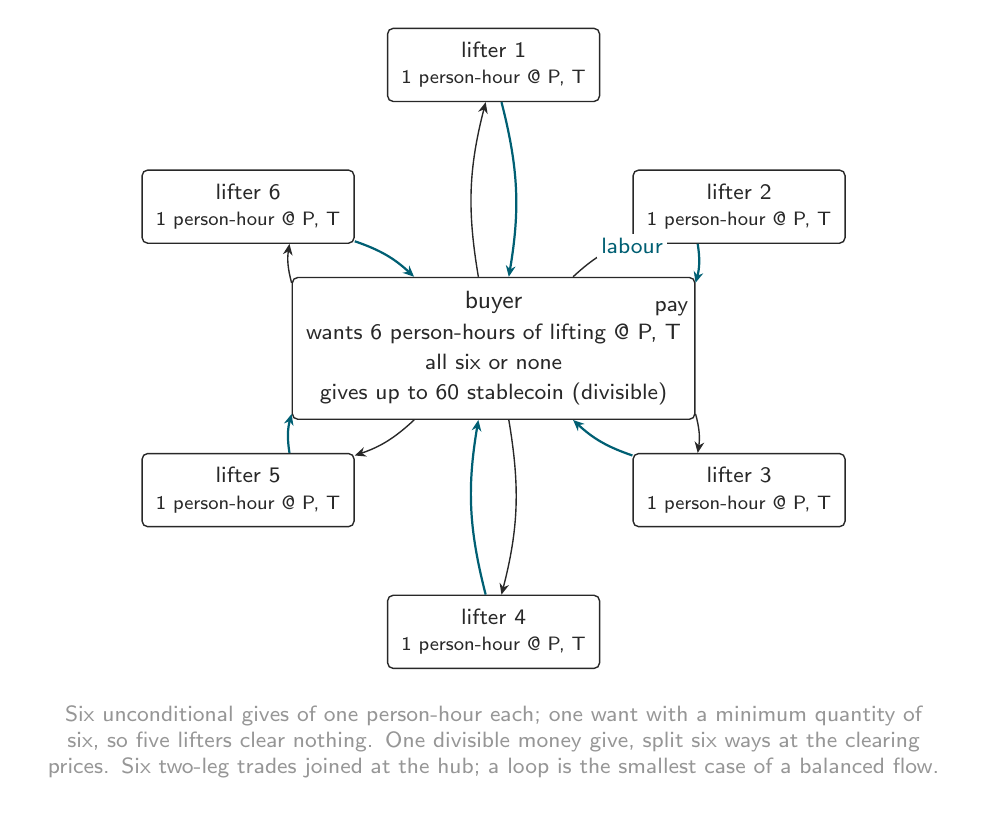
\begin{tikzpicture}
  % Composition by aggregation: six unconditional gives of one person-hour
  % each satisfy one want with a minimum quantity of six. The buyer pays once.
  \node[maker, align=center, minimum width=40mm] (B) at (0,0) {buyer\\{\footnotesize wants 6 person-hours of lifting @ P, T}\\{\footnotesize all six or none}\\{\footnotesize gives up to 60 stablecoin (divisible)}};
  \foreach \i/\a in {1/90,2/30,3/-30,4/-90,5/-150,6/150} {
    \node[maker, font=\footnotesize, minimum width=20mm, align=center] (W\i) at (\a:36mm) {lifter \i\\{\scriptsize 1 person-hour @ P, T}};
    \draw[strong] (W\i) to[bend left=12] (B);
    \draw[flow] (B) to[bend left=12] (W\i);
  }
  \node[lbl, text=accent] at ($(W2)!0.5!(B) + (2mm,4mm)$) {labour};
  \node[lbl] at ($(W2)!0.5!(B) + (7mm,-4mm)$) {pay};
  \node[note, text width=116mm] at (0,-50mm) {Six unconditional gives of one person-hour each; one want with a minimum quantity of six, so five lifters clear nothing. One divisible money give, split six ways at the clearing prices. Six two-leg trades joined at the hub; a loop is the smallest case of a balanced flow.};
\end{tikzpicture}
\end{document}
